\section{Methodology}\label{methodology}

A methodology is a set of methods, rules and restrictions combined to
form a procedure or discipline.

By adhering to a development methodology it is possible to set
development goals and a way to identify trouble areas during a project
allowing for plans and contingencies to be allocated to improve the
likelihood of success.

\subsection{Overview of types of
methodology}\label{overview-of-types-of-methodology}

There are many forms of methodologies, below are a few of the most
popular and an overview of each.

\subsubsection{Rapid Applications Development
(RAD)}\label{rapid-applications-development-rad}

By producing prototypes of the software quickly customers are able to
test and provide feedback as the software is developed. This is useful
as often requirements change and it's common for developers to produce
software that isn't actually what the customer wanted.

\subsubsection{Agile}\label{agile}

Originally project management was slow to adapt to changes with user
review coming in late stages of development. Agile however aims for
incremental development with regular feedback. \parencite{agile}

The most popular form of agile development is the Scrum
\parencite{agile} scrum is suited towards small teams and requires close
involvement by the product owner to provide regular feedback and review.

\subsubsection{Lean}\label{lean}

Much like scrum and other agile methodologies aims to produce software
quickly and involves close coordination with the product owner, where
lean varies is that it wants to reduce waste by selecting the most
valuable features required.\parencite{agilemethods}.

\subsubsection{Waterfall}\label{waterfall}

Focuses on phases such as; requirement gathering, analyses, development
and testing. Each phase is completed entirely before moving onto the
next phase and is often depicted by the phases flowing steadily
downwards resembling a waterfall.

\subsubsection{Spiral}\label{spiral}

The spiral model is based on the incremental model and consists of four
phases; Planning, risk analysis, engineering and evaluation
\parencite{spiral}. A project will go through each phase multiple times
in an iterative process or spirals. This is very well illustrated in the
figure below.

\begin{figure}
\centering
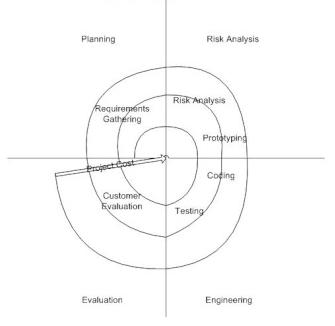
\includegraphics{../../Images/Spiral-model.jpg}
\caption{Spiral model diagram \parencite{spiral}}
\end{figure}

\subsubsection{Time Boxing}\label{time-boxing}

Involves strict deadlines rather than goals. By developing up to the
agreed upon time and evaluating progress this can allow for steadier
development and a set time in mind which provides a deadline for
development.

Evaluating at the end of the time frame can show struggles in the
development process and provides the ability to address them rather than
simply spending more time to complete the goal.

\subsection{Choice of methodology}\label{choice-of-methodology}

After assessing the various forms of project methodologies I have
decided to use an agile methodology most notably the Lean methodology as
this will provide me the ability to develop core functionality in a fast
pace and add other features time permitting. To assist my development I
will also be using time boxing to allocate time for my applications
functions and allow me to perform regular performance reviews so I can
identify time sinks and other issues to allow me to manage them.

\subsection{Project Time line}\label{project-time-line}

Below is a Gantt chart of the overall plan for my project. A Gantt chart
doesn't suit my development methodology very well and so is fairly
high-level overview.

\begin{landscape}
\begin{figure}[htbp]
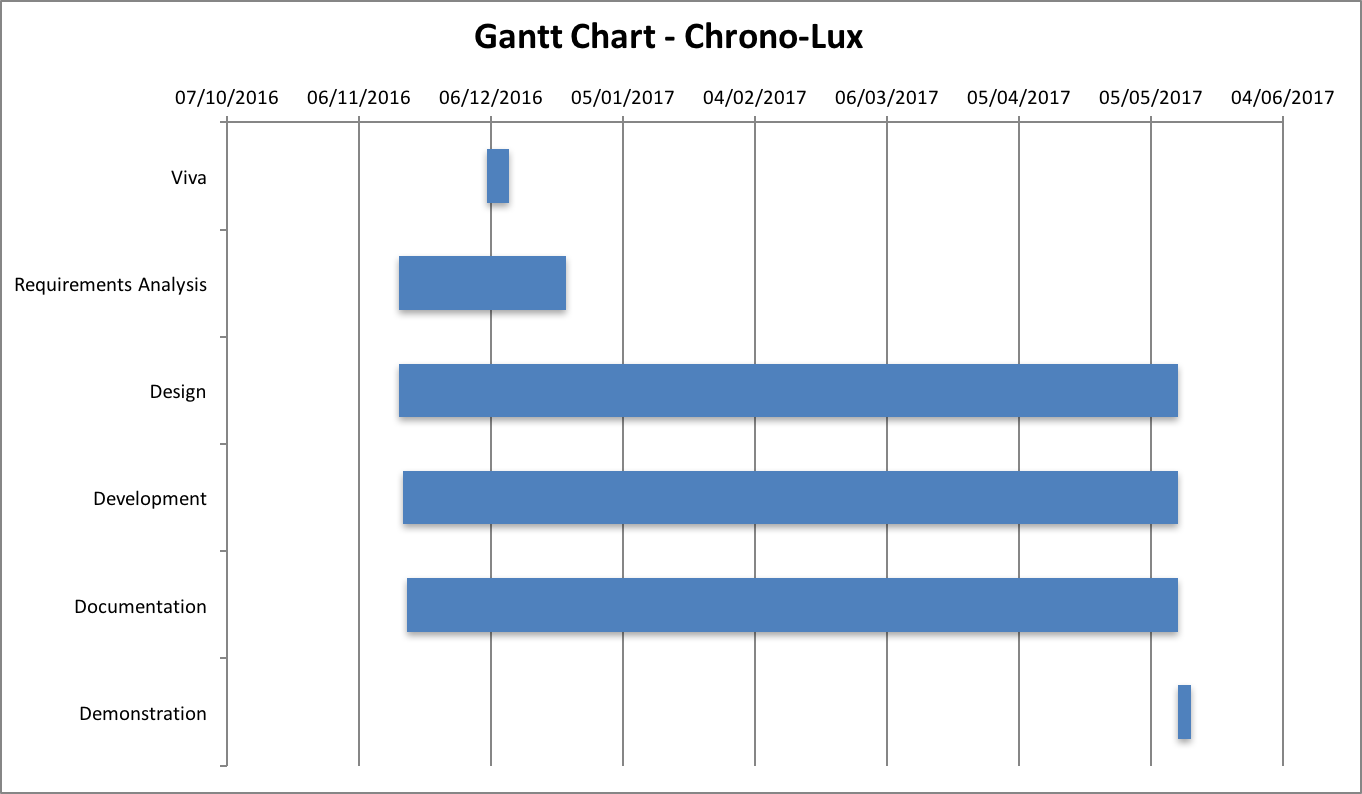
\includegraphics{Images/gantt.png}
\caption{Project Gantt Chart}
\end{figure}
\end{landscape}
